% Options for packages loaded elsewhere
\PassOptionsToPackage{unicode}{hyperref}
\PassOptionsToPackage{hyphens}{url}
%
\documentclass[
  12pt,
]{article}
\usepackage{amsmath,amssymb}
\usepackage{lmodern}
\usepackage{iftex}
\ifPDFTeX
  \usepackage[T1]{fontenc}
  \usepackage[utf8]{inputenc}
  \usepackage{textcomp} % provide euro and other symbols
\else % if luatex or xetex
  \usepackage{unicode-math}
  \defaultfontfeatures{Scale=MatchLowercase}
  \defaultfontfeatures[\rmfamily]{Ligatures=TeX,Scale=1}
  \setmainfont[]{Times New Roman}
\fi
% Use upquote if available, for straight quotes in verbatim environments
\IfFileExists{upquote.sty}{\usepackage{upquote}}{}
\IfFileExists{microtype.sty}{% use microtype if available
  \usepackage[]{microtype}
  \UseMicrotypeSet[protrusion]{basicmath} % disable protrusion for tt fonts
}{}
\makeatletter
\@ifundefined{KOMAClassName}{% if non-KOMA class
  \IfFileExists{parskip.sty}{%
    \usepackage{parskip}
  }{% else
    \setlength{\parindent}{0pt}
    \setlength{\parskip}{6pt plus 2pt minus 1pt}}
}{% if KOMA class
  \KOMAoptions{parskip=half}}
\makeatother
\usepackage{xcolor}
\usepackage[margin=2.54cm]{geometry}
\usepackage{graphicx}
\makeatletter
\def\maxwidth{\ifdim\Gin@nat@width>\linewidth\linewidth\else\Gin@nat@width\fi}
\def\maxheight{\ifdim\Gin@nat@height>\textheight\textheight\else\Gin@nat@height\fi}
\makeatother
% Scale images if necessary, so that they will not overflow the page
% margins by default, and it is still possible to overwrite the defaults
% using explicit options in \includegraphics[width, height, ...]{}
\setkeys{Gin}{width=\maxwidth,height=\maxheight,keepaspectratio}
% Set default figure placement to htbp
\makeatletter
\def\fps@figure{htbp}
\makeatother
\setlength{\emergencystretch}{3em} % prevent overfull lines
\providecommand{\tightlist}{%
  \setlength{\itemsep}{0pt}\setlength{\parskip}{0pt}}
\setcounter{secnumdepth}{5}
\newlength{\cslhangindent}
\setlength{\cslhangindent}{1.5em}
\newlength{\csllabelwidth}
\setlength{\csllabelwidth}{3em}
\newlength{\cslentryspacingunit} % times entry-spacing
\setlength{\cslentryspacingunit}{\parskip}
\newenvironment{CSLReferences}[2] % #1 hanging-ident, #2 entry spacing
 {% don't indent paragraphs
  \setlength{\parindent}{0pt}
  % turn on hanging indent if param 1 is 1
  \ifodd #1
  \let\oldpar\par
  \def\par{\hangindent=\cslhangindent\oldpar}
  \fi
  % set entry spacing
  \setlength{\parskip}{#2\cslentryspacingunit}
 }%
 {}
\usepackage{calc}
\newcommand{\CSLBlock}[1]{#1\hfill\break}
\newcommand{\CSLLeftMargin}[1]{\parbox[t]{\csllabelwidth}{#1}}
\newcommand{\CSLRightInline}[1]{\parbox[t]{\linewidth - \csllabelwidth}{#1}\break}
\newcommand{\CSLIndent}[1]{\hspace{\cslhangindent}#1}
\usepackage{booktabs}
\usepackage{longtable}
\usepackage{array}
\usepackage{multirow}
\usepackage{wrapfig}
\usepackage{float}
\usepackage{colortbl}
\usepackage{pdflscape}
\usepackage{tabu}
\usepackage{threeparttable}
\usepackage{threeparttablex}
\usepackage[normalem]{ulem}
\usepackage{makecell}
\usepackage{xcolor}
\ifLuaTeX
  \usepackage{selnolig}  % disable illegal ligatures
\fi
\IfFileExists{bookmark.sty}{\usepackage{bookmark}}{\usepackage{hyperref}}
\IfFileExists{xurl.sty}{\usepackage{xurl}}{} % add URL line breaks if available
\urlstyle{same} % disable monospaced font for URLs
\hypersetup{
  pdftitle={Insert title of project here},
  pdfauthor={Yixin Fang, Jiahuan Li, Yuxiang Ren, Jinglin Zhang},
  hidelinks,
  pdfcreator={LaTeX via pandoc}}

\title{Insert title of project here}
\usepackage{etoolbox}
\makeatletter
\providecommand{\subtitle}[1]{% add subtitle to \maketitle
  \apptocmd{\@title}{\par {\large #1 \par}}{}{}
}
\makeatother
\subtitle{\url{https://github.com/Artemis20123/FangLiRenZhang_ENV872_EDA_FinalProject}}
\author{Yixin Fang, Jiahuan Li, Yuxiang Ren, Jinglin Zhang}
\date{}

\begin{document}
\maketitle

\newpage
\tableofcontents 
\newpage
\listoftables 
\newpage
\listoffigures 
\newpage

\hypertarget{rationale-and-research-questions}{%
\section{Rationale and Research
Questions}\label{rationale-and-research-questions}}

\newpage

\hypertarget{dataset-information}{%
\section{Dataset Information}\label{dataset-information}}

\hypertarget{data-sources}{%
\subsection{Data sources}\label{data-sources}}

This project relies on two primary datasets. The first dataset, China
\(PM_{2.5}\) pollution data, is available via the Zenodo data
repository\(^{[1]}\). This dataset provides information on the daily
concentration of particulate matter (\(PM_{2.5}\)) in the atmosphere
over China, as measured by satellite sensors. The dataset contains daily
average \(PM_{2.5}\) concentration values for a period from 2000 to
2021, covering the entirety of China's land area. The data is presented
in the form of raster images, with a spatial resolution of 0.01 degrees.
This high-resolution dataset allows for accurate identification of high
pollution cities and regions, and is an important resource for
understanding the severity and extent of air pollution in China.

The second dataset utilized in this project is a shapefile of Chinese
cities boundaries, provided by the statistical bureau of the Chinese
government. The shapefile includes Chinese city names, unique
identifiers, and geometry information for the city polygons. This
dataset enables the mapping of \(PM_{2.5}\) concentrations across
different Chinese cities and supports the time series analysis.
Together, these datasets form the foundation of our dashboard and other
relevant analysis, providing important insights into the spatial and
temporal distribution of \(PM_{2.5}\) pollution in China.

\hypertarget{wrangling-process}{%
\subsection{\texorpdfstring{\href{https://github.com/Artemis20123/FangLiRenZhang_ENV872_EDA_FinalProject/blob/main/Code/data\%20wrangling.Rmd}{Wrangling
process}}{Wrangling process}}\label{wrangling-process}}

The project involves two main data wrangling processes. The first
process involves converting raw NetCDF files to GeoTIFF files using
Python code provided by the dataset creators. The conversion code
utilizes the GDAL package, a translator library for raster and vector
geospatial data formats, to read the SDS data from the NetCDF files,
define missing values, read longitude and latitude information, define
the output file, and write a GeoTIFF file. The NetCDF files are not
included in the repository and can be downloaded from the Zenodo
repository.

In the second data wrangling process, zonal statistics are calculated in
R to aggregate the information of raster pixels within the city boundary
and generate the output as a CSV table. The shapefile with polygon IDs
is loaded, and a list of all raster files in the folder is obtained. A
loop function is used to extract zonal statistics for each raster file,
and two data frames are created to store the sum and mean values of
\$PM\_\{2.5\}\$ concentrations. The zonal function from the terra
package is used to extract the statistics, and the resulting CSV file
contains the daily \$PM\_\{2.5\}\$ information for all the cities.

Finally, all the CSV files containing separate daily \$PM\_\{2.5\}\$
information are aggregated into one large CSV file. Then, the daily
records are summarized to the monthly level to facilitate dashboard
visualization and time series analysis.

\newpage

\hypertarget{exploratory-analysis}{%
\section{Exploratory Analysis}\label{exploratory-analysis}}

To explore the data, we wanted to create a visualization of the monthly
PM2.5 for the cities from 2000 to 2021. The data was first filtered to
include only the seven cities of interest. Then we grouped the data by
city, year, and month and summarized the mean PM2.5 value for each
month. A monthly PM2.5 line plot was created for each city using
ggplot2.

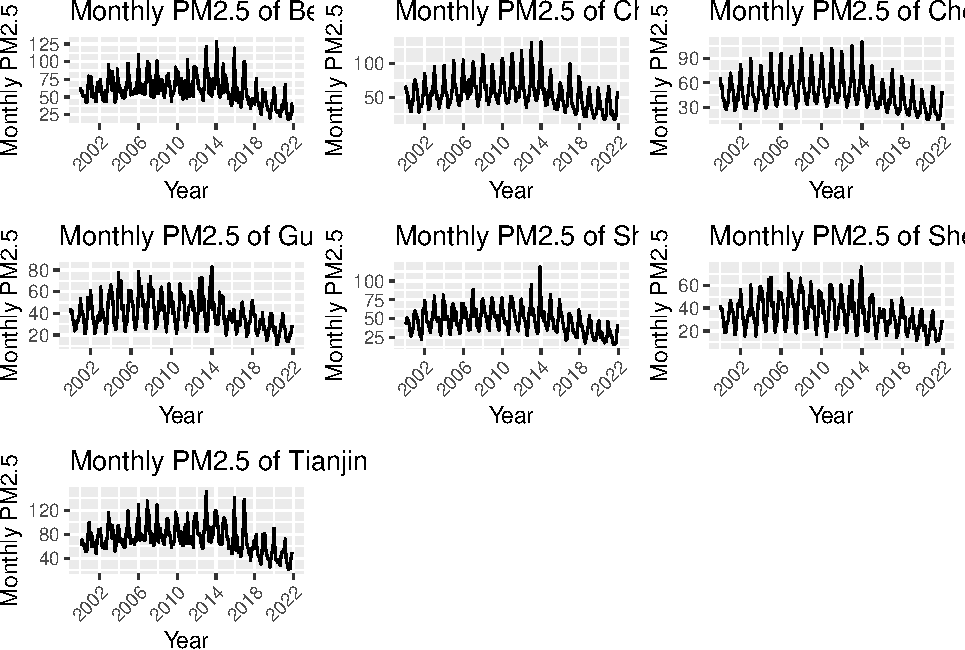
\includegraphics{LiFangRenZhang_ENV872_Project_files/figure-latex/TSA Visualization-1.pdf}

The plot showed that Beijing and Tianjin had the highest PM2.5 values
among the seven cities, and Shenzhen had the lowest values. Most of the
cities seemed to have a slow increase in PM2.5 from 2000 to 2006, then
stayed relatively constant from 2006 until 2014. In 2014, most cities
had a spike in PM2.5. From 2014, PM2.5 in all cities showed a decreasing
trend. To better understand the changes in PM2.5, we conducted
time-series analysis and predicted the monthly PM2.5 for the seven
cities from 2022 to 2026.

\newpage

\hypertarget{analysis}{%
\section{Analysis}\label{analysis}}

\hypertarget{part1-time-series-analysis}{%
\subsection{Part1: Time Series
Analysis}\label{part1-time-series-analysis}}

\hypertarget{seven-cities-monthly-pm2.5-20002021}{%
\subsubsection{Seven cities monthly PM2.5
(2000\textasciitilde2021)}\label{seven-cities-monthly-pm2.5-20002021}}

Using the STL function, we decomposed the PM2.5 time series data of the
target cities into seasonal and trend components and performed a
comparative analysis. The PM2.5 values in these cities are generally
lower during the summer months (June, July, August, and September) and
higher during the winter months (November, December, January, and
February) (Figure 2). There are several possible factors contributing to
this seasonality: First, In the summer, temperatures are higher, leading
to more active air convection, which facilitates the dispersion and
dissipation of pollutants in the air. Secondly, there tends to be more
rainfall in the summer, which can wash PM2.5 particles from the
atmosphere to the ground, reducing their measured values
(\protect\hyperlink{ref-rain}{Pu, Zhao, Zhang, \& Ma, 2011}). Thirdly,
in the winter, heating demand increases, and in some areas, coal
combustion remains the primary method of providing heat
(\protect\hyperlink{ref-heating}{Liang et al., 2015}). This leads to
increased emissions of coal-related pollutants, causing a rise in PM2.5
levels.

\begin{figure}
\centering
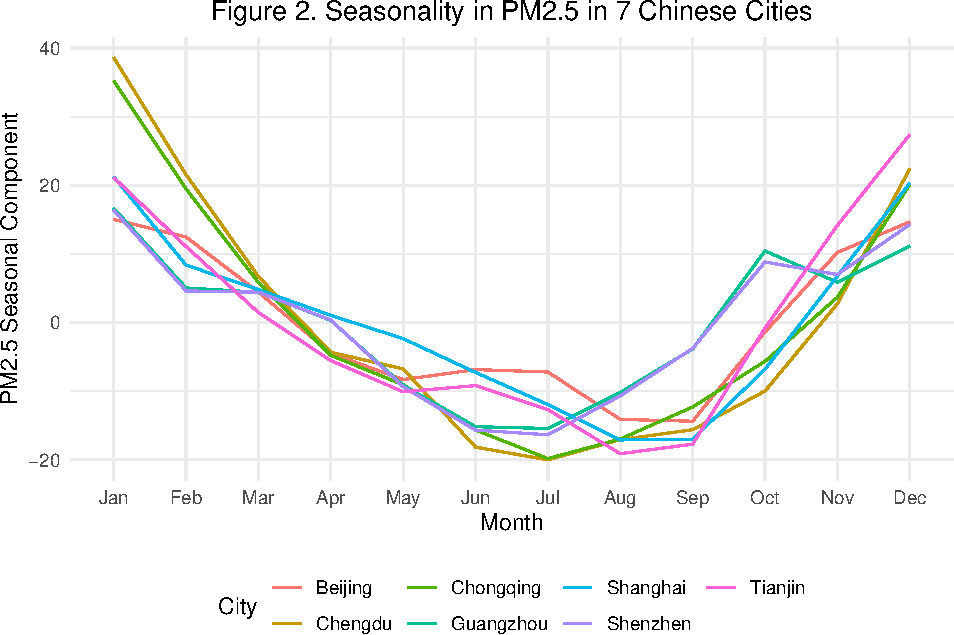
\includegraphics{LiFangRenZhang_ENV872_Project_files/figure-latex/seasonal figure-1.pdf}
\caption{Figure 2. Seasonality in PM2.5 in 7 Chinese Cities}
\end{figure}

The trend results for the target cities are consistent with those
observed in the exploratory analysis (Figure 3). Notably, around 2014
marked a turning point when PM2.5 levels in major cities began to
decrease gradually. This shift is likely attributed to the Chinese
government's implementation of the Air Pollution Prevention and Control
Action Plan, released in September 2013
(\protect\hyperlink{ref-plan}{Cai et al., 2017}). This plan was the
first time the Chinese government set explicit air quality improvement
targets. It required that, by 2017, the annual average PM2.5
concentration in cities at or above the prefectural level should be
reduced by more than 10\%. In key regions such as Beijing-Tianjin-Hebei,
the Yangtze River Delta, and the Pearl River Delta, the plan aimed for
reductions of 25\%, 20\%, and 15\%, respectively.

\begin{figure}
\centering
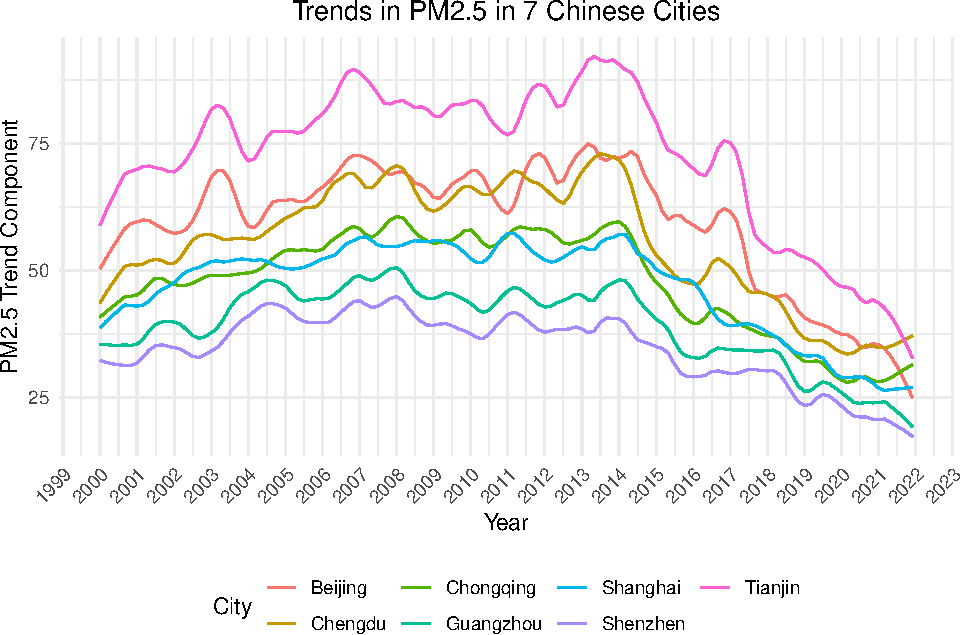
\includegraphics{LiFangRenZhang_ENV872_Project_files/figure-latex/trend figure-1.pdf}
\caption{Figure 3. Trends in PM2.5 in 7 Chinese Cities}
\end{figure}

\hypertarget{seven-cities-monthly-pm2.5-forecast-20222026}{%
\subsubsection{Seven cities monthly PM2.5 forecast
(2022\textasciitilde2026)}\label{seven-cities-monthly-pm2.5-forecast-20222026}}

In order to obtain better forecasting results, we conducted a predictive
accuracy test on multiple time series models based on Beijing's data
from 2000 to 2020 (using actual 2021 data as a benchmark for
comparison). These models include:

\begin{enumerate}
\def\labelenumi{\arabic{enumi}.}
\tightlist
\item
  Arithmetic Mean Model (Mean): This model assumes that future
  observations will equal current observations, i.e., the predicted
  future value equals the current value, making the model a constant
  average value model.
\item
  Seasonal Naive Model (SNAIVE): It assumes that future observations
  will equal the most recent observations from the same season. The
  model focuses solely on historical data within the same season.
\item
  Seasonal Autoregressive Integrated Moving Average Model (SARIMA):
  SARIMA is a widely-used seasonal time series model that builds upon
  the ARIMA model by incorporating seasonal variations in the time
  series data.
\item
  Seasonal Simple Exponential Smoothing (SSES) Model: This is a time
  series forecasting method based on weighted averages.
\end{enumerate}

In these four models tested, the SSES model had the smallest Root Mean
Square Error (RMSE) and the best forecasting capability (Table 1).
However, considering that the forecasting target is for the next five
years, both SSES and SNAIVE models predict the same values for the
first, second, third, fourth, and fifth years when forecasting multiple
years. As a result, we combined the results of SSES and SNAIVE with the
SARIMA model, creating two new models:

\begin{table}

\caption{\label{tab:accuacy_table1}Forecast Accuracy for Seasonal Data}
\centering
\begin{tabular}[t]{l|r|r|r|r|r}
\hline
  & ME & RMSE & MAE & MPE & MAPE\\
\hline
MEAN & -28.1059 & 31.6898 & 29.2560 & -119.0707 & 120.7650\\
\hline
SNAIVE & -2.4987 & 13.4377 & 9.3796 & -17.3618 & 28.6924\\
\hline
SARIMA & -4.3333 & 14.5863 & 12.2154 & -32.3573 & 45.6127\\
\hline
\cellcolor{gray!6}{SSES} & \cellcolor{gray!6}{4.8008} & \cellcolor{gray!6}{12.3008} & \cellcolor{gray!6}{7.7936} & \cellcolor{gray!6}{5.2446} & \cellcolor{gray!6}{19.6416}\\
\hline
\end{tabular}
\end{table}

\begin{enumerate}
\def\labelenumi{\arabic{enumi}.}
\setcounter{enumi}{4}
\tightlist
\item
  SNAIVE\_SARIMA. The average of SNAIVE and SARIMA.
\item
  SSES\_SARIMA. The average of SSES and SARIMA.
\end{enumerate}

Although the accuracy results show that the RMSE of SSES\_SARIMA is the
second smallest, its predictive accuracy is still slightly lower than
that of SSES (Table 2). However, considering the forecasting objective
and the comparison with other models, we ultimately chose to use the
SSES\_SARIMA model for predicting PM2.5 levels in the target cities.

\begin{table}

\caption{\label{tab:accuacy_table2}Forecast Accuracy for Seasonal Data}
\centering
\begin{tabular}[t]{l|r|r|r|r|r}
\hline
  & ME & RMSE & MAE & MPE & MAPE\\
\hline
MEAN & -28.105858 & 31.68980 & 29.256003 & -119.070730 & 120.76499\\
\hline
SNAIVE & -2.498701 & 13.43770 & 9.379570 & -17.361823 & 28.69245\\
\hline
SARIMA & -4.333324 & 14.58628 & 12.215420 & -32.357291 & 45.61268\\
\hline
\cellcolor{gray!6}{SSES} & \cellcolor{gray!6}{4.800801} & \cellcolor{gray!6}{12.30076} & \cellcolor{gray!6}{7.793640} & \cellcolor{gray!6}{5.244604} & \cellcolor{gray!6}{19.64161}\\
\hline
SNAIVE\_SARIMA & -3.416013 & 13.00090 & 9.967983 & -24.859557 & 35.26887\\
\hline
SSES\_SARIMA & 0.233739 & 12.50184 & 9.574127 & -13.556343 & 31.19364\\
\hline
\end{tabular}
\end{table}

\hypertarget{question-2}{%
\subsection{Question 2:}\label{question-2}}

To better visualize the data, we created a dashboard using Shiny. The
dashboard consisted of three side panels:``PM2.5 National
Distribution'', ``Time Series Visualization by City'', ``PM2.5
Prediction by City'' and three corresponding tab panels: ``Map'',
``TSA'', and ``Prediction''.

The ``PM2.5 National Distribution'' allows users to drag the map in the
``Map'' tab and explore the PM2.5 distribution pattern in the country.
The ``Time Series Visualization by City'' panel has a dropdown box that
allows users to select the monthly PM2.5 visualization of each city. The
results are displayed in the ``TSA'' tab. Finally, the ``PM2.5
Prediction by City'' panel has a dropdown box and slider. Users can
select the city and the time range to view the monthly PM2.5 prediction
in the ``Prediction'' tab.

\newpage

\hypertarget{summary-and-conclusions}{%
\section{Summary and Conclusions}\label{summary-and-conclusions}}

\newpage

\hypertarget{references}{%
\section{References}\label{references}}

{[}1{]} Wei, J., Li, Z., Lyapustin, A., Sun, L., Peng, Y., Xue, W., Su,
T., and Cribb, M. Reconstructing 1-km-resolution high-quality
PM\textsubscript{2.5}~data records from 2000 to 2018 in China:
spatiotemporal variations and policy implications.~\emph{Remote Sensing
of Environment}, 2021, 252, 112136.
\url{https://doi.org/10.1016/j.rse.2020.112136}

\hypertarget{refs}{}
\begin{CSLReferences}{1}{0}
\leavevmode\vadjust pre{\hypertarget{ref-plan}{}}%
Cai, S., Wang, Y., Zhao, B., Wang, S., Chang, X., \& Hao, J. (2017). The
impact of the {``air pollution prevention and control action plan''} on
PM2. 5 concentrations in jing-jin-ji region during 2012--2020.
\emph{Science of the Total Environment}, \emph{580}.

\leavevmode\vadjust pre{\hypertarget{ref-heating}{}}%
Liang, X., Zou, T., Guo, B., Li, S., Zhang, H., Zhang, S., \ldots{}
Chen, S. X. (2015). Assessing beijing's PM2. 5 pollution: Severity,
weather impact, APEC and winter heating. \emph{Proceedings of the Royal
Society A: Mathematical, Physical and Engineering Sciences}, \emph{471}.

\leavevmode\vadjust pre{\hypertarget{ref-rain}{}}%
Pu, W., Zhao, X., Zhang, X., \& Ma, Z. (2011). Effect of meteorological
factors on PM2. 5 during july to september of beijing. \emph{Procedia
Earth and Planetary Science}, \emph{2}, 272--277.

\end{CSLReferences}

\end{document}
